% =====================================================================
% CHAPTER 5 -- Summary of: C. Sabato, Master's thesis, Politecnico di Torino, 2025 [Sabato2025]
% =====================================================================
\section*{CHAPTER 5. 60 GHz SES DESIGN AND DEPLOYMENT}
\addcontentsline{toc}{section}{\numberline{}CHAPTER 5. 60 GHz SES DESIGN AND DEPLOYMENT}
\setcounter{section}{5}
\setcounter{subsection}{0}
\setcounter{equation}{0}
\setcounter{theorem}{0}
\setcounter{figure}{0}
\setcounter{table}{0}

\subsection{Problem}
At 60~GHz, indoor links suffer from high path loss and are easily blocked by walls. In the reference laboratory, two rooms are separated by a partial wall, so a transmitter in one room leaves the other room in shadow (Fig.~\ref{fig:ch5-scenario})~\cite{Sabato2025}. The thesis asks two questions. How can passive SESs restore coverage in this non-line-of-sight (NLOS) area? And can they also support passive localization? If the angular response of each SES is known, the sector from which a terminal transmits can be identified~\cite{Sabato2025}.

\subsection{Contributions and Methodology}
Sabato~\cite{Sabato2025} builds a complete design flow for passive 60~GHz SESs and applies it to a real laboratory:
\begin{itemize}
    \item \textbf{Unit cell and substrate.} The cell is a square patch on a grounded single-layer PCB, about $\lambda/2$ wide at 60~GHz. It was analysed with Floquet ports in CST for patch widths of 0.2--2.4~mm at 58, 60 and 62~GHz.
    \begin{itemize}
        \item FR4 ($\varepsilon_r = 4.2$--4.8, $\tan\delta = 0.02$--0.025) is rejected for its high losses in favour of Rogers RO3003 ($\varepsilon_r = 3.0$, $\tan\delta = 0.0010$).
        \item The 0.13 and 0.25~mm laminates exceed $360^\circ$ of phase, but their steep phase slopes and resonance spikes make them sensitive to fabrication errors.
        \item The 0.76~mm laminate reaches only about $300^\circ$.
        \item The 0.51~mm laminate gives a smooth, full $360^\circ$ that stays stable for incidence angles of $0^\circ$--$50^\circ$, so it is selected.
    \end{itemize}
    \item \textbf{Phase synthesis.} To redirect a plane wave arriving from $(\theta_I, \phi_I)$ towards $(\theta_b, \phi_b)$, the $i$-th cell must provide the reflection phase
    \begin{equation}\label{eq:ch5-phase}
    \varphi_R(x_i,y_i) = -k_0\left[\sin\theta_b\left(x_i\cos\phi_b + y_i\sin\phi_b\right) + \sin\theta_I\left(x_i\cos\phi_I + y_i\sin\phi_I\right)\right],
    \end{equation}
    where $(x_i, y_i)$ is the cell position and $k_0$ the free-space wavenumber. The first term tilts the reflected wavefront and the second removes the phase of the incident plane wave~\cite{Sabato2025}. The phases from \eqref{eq:ch5-phase} are converted to patch widths by interpolating the 60~GHz phase curve. The resulting layout is exported from MATLAB as a DXF file and simulated in CST.
    \item \textbf{Validation and deployment.}
    \begin{itemize}
        \item Test arrays of $10 \times 10$ cells ($5\lambda$ side) and $24 \times 24$ cells ($12\lambda$ side) steer a normally incident wave to $\theta_b = 30^\circ$.
        \item In the laboratory, the SES positions are selected by MATLAB ray tracing with up to two reflections. The transmitter is a $2 \times 8$ patch array that steers over $\pm 54^\circ$ in azimuth and to $-18^\circ$, $0^\circ$ or $+18^\circ$ in elevation. The arrangement with the least spillover between surfaces is kept.
        \item Eight SESs of $20 \times 20$ cells are then designed for their angles of arrival and departure and simulated over 58--62~GHz.
    \end{itemize}
\end{itemize}

\begin{figure}[!htbp]
    \centering
    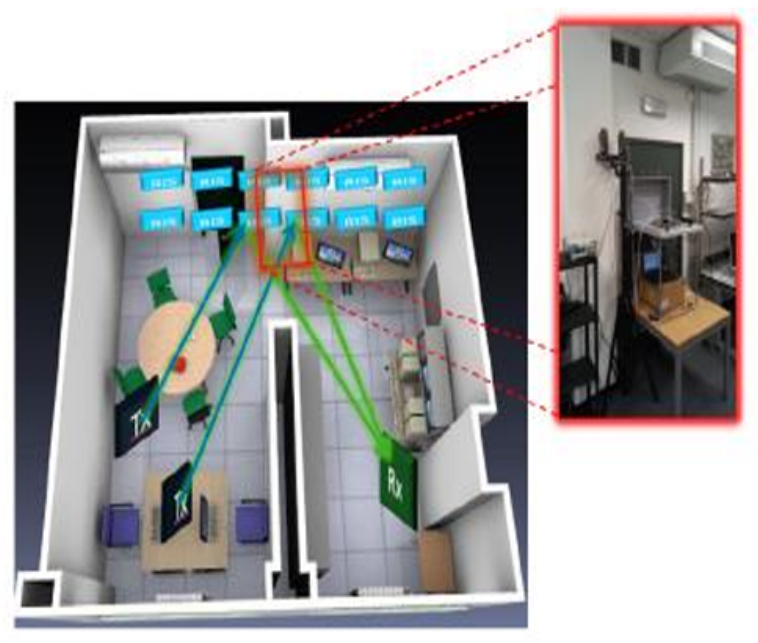
\includegraphics[width=0.6\textwidth]{Images/ch5_sabato_fig4-1-1.png}
    \caption[Indoor reference scenario with multiple SESs]{Indoor reference scenario: two rooms separated by a partial wall, with transmitter (Tx) and receiver (Rx) positions and multiple SESs; the inset shows the real laboratory (adapted from~\cite{Sabato2025}).}
    \label{fig:ch5-scenario}
\end{figure}

\subsection{Limitations of the Approach}
\begin{itemize}
    \item The work relies only on simulation (full-wave CST and ray tracing); no SES was fabricated or measured.
    \item Equation~\eqref{eq:ch5-phase} assumes plane-wave (far-field) illumination, although indoor SESs are often in the near field of the transmitter (see Chapter~4).
    \item The arrays are small ($20 \times 20$ cells, i.e., $10\lambda \times 10\lambda$), which limits directivity. In addition, the phase map is exact only at the 60~GHz design frequency.
    \item Localization is discussed only qualitatively; no localization accuracy is evaluated.
\end{itemize}

\subsection{Results and Evaluation}
\begin{itemize}
    \item \textbf{Test array.} The $24 \times 24$ SES redirects the beam to the designed $30^\circ$~\cite{Sabato2025}. Its side lobes grow from 58 to 62~GHz. At 62~GHz three lobes reach similar levels: the desired beam, the specular reflection of the incident wave, and a lobe mirroring the desired direction. This is expected, since the phase curve is matched only at 60~GHz.
    \item \textbf{Placement.} The W-shaped arrangement of the surfaces gives the least spillover between neighbouring SESs.
    \item \textbf{Eight SESs.} Their simulated main-lobe and side-lobe levels at 60~GHz are listed in Table~\ref{tab:ch5-ses}.
    \begin{itemize}
        \item Six surfaces (SES~2--4 and 6--8) point correctly, with main lobes between $-3$ and $+1$~dB and side lobes 10--16~dB lower.
        \item SES~1 reaches only about $-12$~dB and is slightly mis-pointed in azimuth and elevation, which the author attributes to the finite array size and discretization.
        \item SES~4 has more side lobes because its phase curve is truncated.
        \item SES~5 must steer to $\theta_b = -62^\circ$, so part of its energy leaks into a specular lobe of about $-5$~dB.
    \end{itemize}
    \item \textbf{Frequency robustness.} Over 58--62~GHz, SES~3, 4 and 7 keep their pointing with only small power changes, whereas SES~1, 5 and 6 drift or develop strong specular and side lobes. Performance therefore depends strongly on the steering angle and the array size.
\end{itemize}

\begin{table}[!htbp]
    \centering
    \caption[Simulated performance of the eight SESs at 60 GHz]{Main-lobe and side-lobe levels of the eight SESs at 60~GHz, read from the simulated 2D RCS cuts reported in~\cite{Sabato2025}.}
    \label{tab:ch5-ses}
    \small
    \begin{tabularx}{\textwidth}{c c c >{\raggedright\arraybackslash}X}
        \toprule
        SES & Main lobe (dB) & Side lobes (dB) & Remark \\
        \midrule
        1 & $\approx -12$ & $\leq -25$ & slight mis-pointing, low reflected power \\
        2 & $\approx 0$ & $\approx -12$ & correct pointing \\
        3 & $\approx +1$ & $\approx -12$ & correct pointing, stable over 58--62~GHz \\
        4 & $\approx -3$ & $\approx -13$ & more side lobes (phase-curve truncation) \\
        5 & not reported & -- & extreme angle $\theta_b = -62^\circ$, specular lobe $\approx -5$~dB \\
        6 & $\approx -1$ & $\approx -17$ & stronger specular and mirror lobes \\
        7 & $\approx 0$ & $\approx -13$ & correct pointing, stable over 58--62~GHz \\
        8 & $\approx 0$ & $\approx -13$ & correct pointing, weak specular lobe \\
        \bottomrule
    \end{tabularx}
\end{table}

\subsection{Open Issues and Future Directions}
The author proposes full-wave simulations of the whole environment (e.g., with HFSS) and measurements on fabricated SESs, to close the gap between theory and practice~\cite{Sabato2025}. The results point to four further steps:
\begin{itemize}
    \item near-field-aware synthesis for SESs close to the transmitter, as in Chapter~4;
    \item larger apertures to raise the main lobe of weak surfaces such as SES~1;
    \item phase compensation over 58--62~GHz to limit side-lobe growth;
    \item an experimental test of the localization concept with a quantified accuracy.
\end{itemize}
